\documentclass[11pt,preprint, authoryear]{elsarticle}

\usepackage{lmodern}
%%%% My spacing
\usepackage{setspace}
\setstretch{1.2}
\DeclareMathSizes{12}{14}{10}{10}

% Wrap around which gives all figures included the [H] command, or places it "here". This can be tedious to code in Rmarkdown.
\usepackage{float}
\let\origfigure\figure
\let\endorigfigure\endfigure
\renewenvironment{figure}[1][2] {
    \expandafter\origfigure\expandafter[H]
} {
    \endorigfigure
}

\let\origtable\table
\let\endorigtable\endtable
\renewenvironment{table}[1][2] {
    \expandafter\origtable\expandafter[H]
} {
    \endorigtable
}


\usepackage{ifxetex,ifluatex}
\usepackage{fixltx2e} % provides \textsubscript
\ifnum 0\ifxetex 1\fi\ifluatex 1\fi=0 % if pdftex
  \usepackage[T1]{fontenc}
  \usepackage[utf8]{inputenc}
\else % if luatex or xelatex
  \ifxetex
    \usepackage{mathspec}
    \usepackage{xltxtra,xunicode}
  \else
    \usepackage{fontspec}
  \fi
  \defaultfontfeatures{Mapping=tex-text,Scale=MatchLowercase}
  \newcommand{\euro}{€}
\fi

\usepackage{amssymb, amsmath, amsthm, amsfonts}

\def\bibsection{\section*{References}} %%% Make "References" appear before bibliography


\usepackage[round]{natbib}

\usepackage{longtable}
\usepackage[margin=2.3cm,bottom=2cm,top=2.5cm, includefoot]{geometry}
\usepackage{fancyhdr}
\usepackage[bottom, hang, flushmargin]{footmisc}
\usepackage{graphicx}
\numberwithin{equation}{section}
\numberwithin{figure}{section}
\numberwithin{table}{section}
\setlength{\parindent}{0cm}
\setlength{\parskip}{1.3ex plus 0.5ex minus 0.3ex}
\usepackage{textcomp}
\renewcommand{\headrulewidth}{0.2pt}
\renewcommand{\footrulewidth}{0.3pt}

\usepackage{array}
\newcolumntype{x}[1]{>{\centering\arraybackslash\hspace{0pt}}p{#1}}

%%%%  Remove the "preprint submitted to" part. Don't worry about this either, it just looks better without it:
\makeatletter
\def\ps@pprintTitle{%
  \let\@oddhead\@empty
  \let\@evenhead\@empty
  \let\@oddfoot\@empty
  \let\@evenfoot\@oddfoot
}
\makeatother

 \def\tightlist{} % This allows for subbullets!

\usepackage{hyperref}
\hypersetup{breaklinks=true,
            bookmarks=true,
            colorlinks=true,
            citecolor=blue,
            urlcolor=blue,
            linkcolor=blue,
            pdfborder={0 0 0}}


% The following packages allow huxtable to work:
\usepackage{siunitx}
\usepackage{multirow}
\usepackage{hhline}
\usepackage{calc}
\usepackage{tabularx}
\usepackage{booktabs}
\usepackage{caption}


\newenvironment{columns}[1][]{}{}

\newenvironment{column}[1]{\begin{minipage}{#1}\ignorespaces}{%
\end{minipage}
\ifhmode\unskip\fi
\aftergroup\useignorespacesandallpars}

\def\useignorespacesandallpars#1\ignorespaces\fi{%
#1\fi\ignorespacesandallpars}

\makeatletter
\def\ignorespacesandallpars{%
  \@ifnextchar\par
    {\expandafter\ignorespacesandallpars\@gobble}%
    {}%
}
\makeatother

\newlength{\cslhangindent}
\setlength{\cslhangindent}{1.5em}
\newenvironment{CSLReferences}%
  {\setlength{\parindent}{0pt}%
  \everypar{\setlength{\hangindent}{\cslhangindent}}\ignorespaces}%
  {\par}


\urlstyle{same}  % don't use monospace font for urls
\setlength{\parindent}{0pt}
\setlength{\parskip}{6pt plus 2pt minus 1pt}
\setlength{\emergencystretch}{3em}  % prevent overfull lines
\setcounter{secnumdepth}{5}

%%% Use protect on footnotes to avoid problems with footnotes in titles
\let\rmarkdownfootnote\footnote%
\def\footnote{\protect\rmarkdownfootnote}
\IfFileExists{upquote.sty}{\usepackage{upquote}}{}

%%% Include extra packages specified by user

%%% Hard setting column skips for reports - this ensures greater consistency and control over the length settings in the document.
%% page layout
%% paragraphs
\setlength{\baselineskip}{12pt plus 0pt minus 0pt}
\setlength{\parskip}{12pt plus 0pt minus 0pt}
\setlength{\parindent}{0pt plus 0pt minus 0pt}
%% floats
\setlength{\floatsep}{12pt plus 0 pt minus 0pt}
\setlength{\textfloatsep}{20pt plus 0pt minus 0pt}
\setlength{\intextsep}{14pt plus 0pt minus 0pt}
\setlength{\dbltextfloatsep}{20pt plus 0pt minus 0pt}
\setlength{\dblfloatsep}{14pt plus 0pt minus 0pt}
%% maths
\setlength{\abovedisplayskip}{12pt plus 0pt minus 0pt}
\setlength{\belowdisplayskip}{12pt plus 0pt minus 0pt}
%% lists
\setlength{\topsep}{10pt plus 0pt minus 0pt}
\setlength{\partopsep}{3pt plus 0pt minus 0pt}
\setlength{\itemsep}{5pt plus 0pt minus 0pt}
\setlength{\labelsep}{8mm plus 0mm minus 0mm}
\setlength{\parsep}{\the\parskip}
\setlength{\listparindent}{\the\parindent}
%% verbatim
\setlength{\fboxsep}{5pt plus 0pt minus 0pt}


% code to insert to fix environment Shaded undefined issue with
% showing code chunks in rticle IEEE template.
\usepackage{color}
\usepackage{fancyvrb}
\newcommand{\VerbBar}{|}
\newcommand{\VERB}{\Verb[commandchars=\\\{\}]}
\DefineVerbatimEnvironment{Highlighting}{Verbatim}{commandchars=\\\{\}}
% Add ',fontsize=\small' for more characters per line
\usepackage{framed}
\definecolor{shadecolor}{RGB}{248,248,248}
\newenvironment{Shaded}{\begin{snugshade}}{\end{snugshade}}
\newcommand{\AlertTok}[1]{\textcolor[rgb]{0.94,0.16,0.16}{#1}}
\newcommand{\AnnotationTok}[1]{\textcolor[rgb]{0.56,0.35,0.01}{\textbf{\textit{#1}}}}
\newcommand{\AttributeTok}[1]{\textcolor[rgb]{0.77,0.63,0.00}{#1}}
\newcommand{\BaseNTok}[1]{\textcolor[rgb]{0.00,0.00,0.81}{#1}}
\newcommand{\BuiltInTok}[1]{#1}
\newcommand{\CharTok}[1]{\textcolor[rgb]{0.31,0.60,0.02}{#1}}
\newcommand{\CommentTok}[1]{\textcolor[rgb]{0.56,0.35,0.01}{\textit{#1}}}
\newcommand{\CommentVarTok}[1]{\textcolor[rgb]{0.56,0.35,0.01}{\textbf{\textit{#1}}}}
\newcommand{\ConstantTok}[1]{\textcolor[rgb]{0.00,0.00,0.00}{#1}}
\newcommand{\ControlFlowTok}[1]{\textcolor[rgb]{0.13,0.29,0.53}{\textbf{#1}}}
\newcommand{\DataTypeTok}[1]{\textcolor[rgb]{0.13,0.29,0.53}{#1}}
\newcommand{\DecValTok}[1]{\textcolor[rgb]{0.00,0.00,0.81}{#1}}
\newcommand{\DocumentationTok}[1]{\textcolor[rgb]{0.56,0.35,0.01}{\textbf{\textit{#1}}}}
\newcommand{\ErrorTok}[1]{\textcolor[rgb]{0.64,0.00,0.00}{\textbf{#1}}}
\newcommand{\ExtensionTok}[1]{#1}
\newcommand{\FloatTok}[1]{\textcolor[rgb]{0.00,0.00,0.81}{#1}}
\newcommand{\FunctionTok}[1]{\textcolor[rgb]{0.00,0.00,0.00}{#1}}
\newcommand{\ImportTok}[1]{#1}
\newcommand{\InformationTok}[1]{\textcolor[rgb]{0.56,0.35,0.01}{\textbf{\textit{#1}}}}
\newcommand{\KeywordTok}[1]{\textcolor[rgb]{0.13,0.29,0.53}{\textbf{#1}}}
\newcommand{\NormalTok}[1]{#1}
\newcommand{\OperatorTok}[1]{\textcolor[rgb]{0.81,0.36,0.00}{\textbf{#1}}}
\newcommand{\OtherTok}[1]{\textcolor[rgb]{0.56,0.35,0.01}{#1}}
\newcommand{\PreprocessorTok}[1]{\textcolor[rgb]{0.56,0.35,0.01}{\textit{#1}}}
\newcommand{\RegionMarkerTok}[1]{#1}
\newcommand{\SpecialCharTok}[1]{\textcolor[rgb]{0.00,0.00,0.00}{#1}}
\newcommand{\SpecialStringTok}[1]{\textcolor[rgb]{0.31,0.60,0.02}{#1}}
\newcommand{\StringTok}[1]{\textcolor[rgb]{0.31,0.60,0.02}{#1}}
\newcommand{\VariableTok}[1]{\textcolor[rgb]{0.00,0.00,0.00}{#1}}
\newcommand{\VerbatimStringTok}[1]{\textcolor[rgb]{0.31,0.60,0.02}{#1}}
\newcommand{\WarningTok}[1]{\textcolor[rgb]{0.56,0.35,0.01}{\textbf{\textit{#1}}}}


\begin{document}



\begin{frontmatter}  %

\title{Cross Section Assignment}

% Set to FALSE if wanting to remove title (for submission)




\author[Add1]{Jacques Rossouw}
\ead{gerardrossouw@gmail.com}





\address[Add1]{Stellebosch, Western Cape, South Africa}



\vspace{1cm}





\vspace{0.5cm}

\end{frontmatter}


\newpage
\renewcommand{\contentsname}{Table of Contents}
{\tableofcontents}

%________________________
% Header and Footers
%%%%%%%%%%%%%%%%%%%%%%%%%%%%%%%%%
\pagestyle{fancy}
\chead{}
\rhead{}
\lfoot{}
\rfoot{\footnotesize Page \thepage}
\lhead{}
%\rfoot{\footnotesize Page \thepage } % "e.g. Page 2"
\cfoot{}

%\setlength\headheight{30pt}
%%%%%%%%%%%%%%%%%%%%%%%%%%%%%%%%%
%________________________

\headsep 35pt % So that header does not go over title




\newpage

\hypertarget{introduction}{%
\section{Introduction}\label{introduction}}

The effects of the covid-19 corona virus has led to global economic
strain and the debate over whether strict lockdown rules were necessary
inspite of their economic implications is debated by some.

The problem with identifying the effect that covid policy stringency had
on covid-19 is with the idiosynctratic differences between countries
that also contributed to the severity of how covid would have affected
individuals. This suggests that the fixed effects regression technique
offers a unique opportunity to account for these fixed effects between
countries, and to isolate the effect that policy had on covid. Towards
fighting the coronavirus as a different flu from the typical cold, the
amount of people hospitalised, those ending up in ICU, or deaths per
unit of time is measured relative to the amount of new cases. The
typical flu also spreads rapidly but the the problem is set up as
mentioned, to isolate the effect over and above being a standard flu.

By using the data from H. Ritchie
(\protect\hyperlink{ref-dataset}{2020}), the data is first cleaned by
filtering for only the country components, and removing the countries
for which data does not exist after a certain date.

\hypertarget{data-cleaningfeature-selection}{%
\section{Data Cleaning/Feature
Selection}\label{data-cleaningfeature-selection}}

Some transformations are also made to columns to make them more usable
for regression. The variables that are distributed on a wider range, or
scale, are also scaled to ensure that the OLS estimation is not biased
by this. The code in the \protect\hyperlink{appendix}{Appendix}
illustrates this.

\hypertarget{converting-to-cumulative-values}{%
\subsection{Converting to Cumulative
Values}\label{converting-to-cumulative-values}}

\begin{Shaded}
\begin{Highlighting}[]
\CommentTok{\# See appendix}
\NormalTok{world\_df }\OtherTok{\textless{}{-}}\NormalTok{ world\_df }\SpecialCharTok{\%\textgreater{}\%} \FunctionTok{scale\_bigs\_cumsum}\NormalTok{(.)}
\end{Highlighting}
\end{Shaded}

\hypertarget{variable-features-scaling}{%
\subsection{Variable Features Scaling}\label{variable-features-scaling}}

\begin{verbatim}
##                        mean         sd   min         max       range
## new_cases         261519.32 1220518.92  0.00 25275423.00 25275423.00
## afflicted_rate        26.00      85.81  0.00      931.54      931.54
## reproduction_rate      0.77       0.44 -0.01        2.06        2.08
## new_tests            487.10    1789.23  0.00    32919.30    32919.30
## new_vaccinations     275.41     558.44  0.00     3041.92     3041.92
## stringency_index      44.81      25.15  0.00       99.06       99.06
\end{verbatim}

Thus, want to scale: \texttt{new\_test,\ new\_vaccinations}

Plotting to see whether there is any irregularity in the distribution of
the dependent variable.

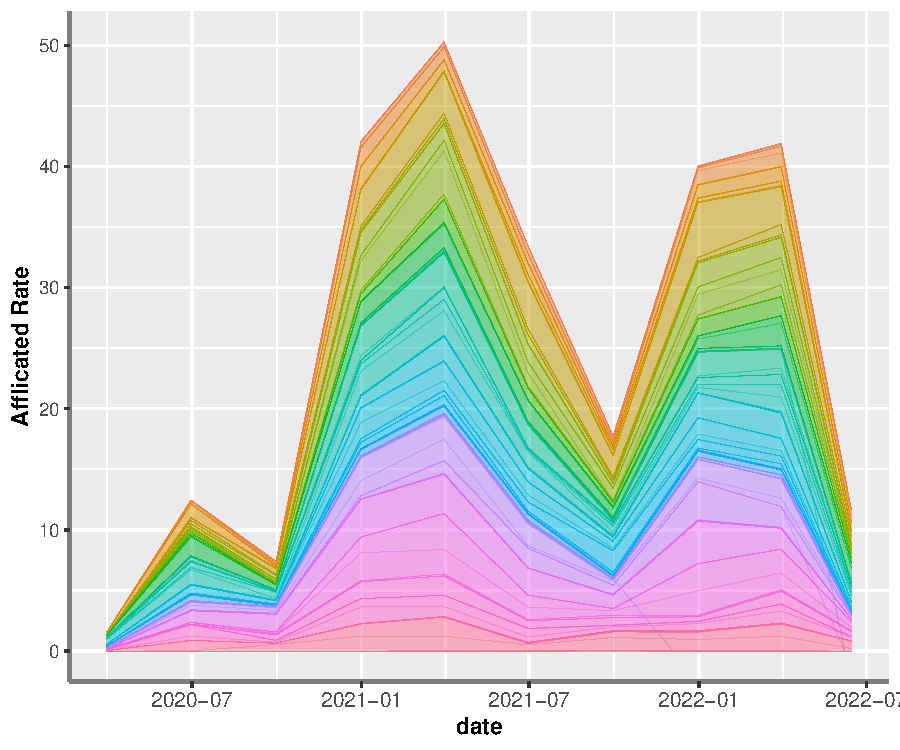
\includegraphics{Cross_Section_Assignment_files/figure-latex/afflicted-1.pdf}

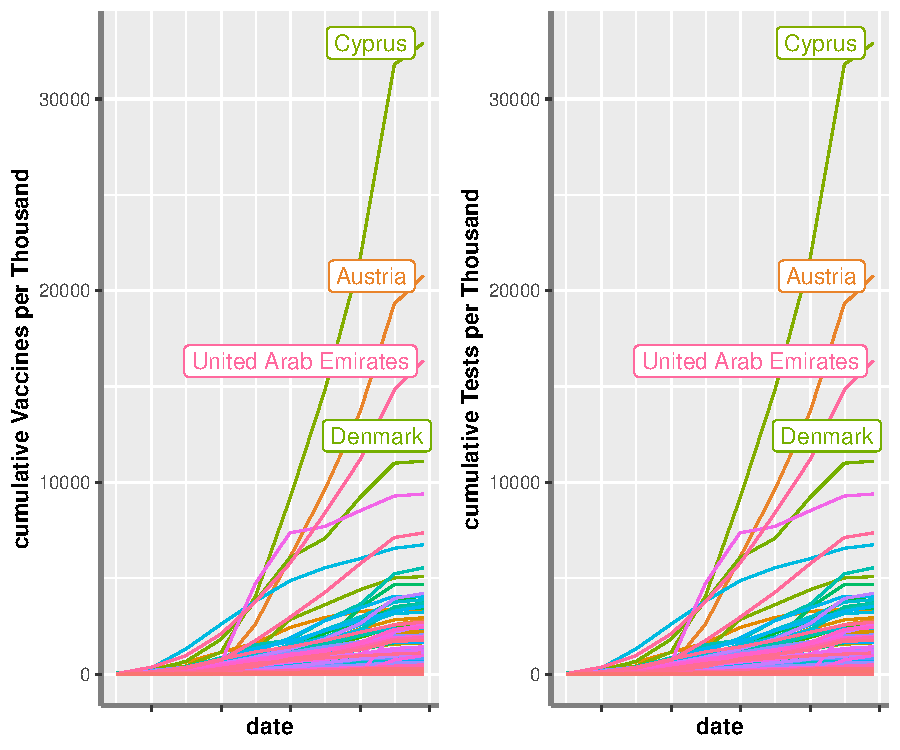
\includegraphics{Cross_Section_Assignment_files/figure-latex/var_plot-1.pdf}

\begin{Shaded}
\begin{Highlighting}[]
\NormalTok{world\_df }\OtherTok{\textless{}{-}}\NormalTok{ world\_df }\SpecialCharTok{\%\textgreater{}\%} \FunctionTok{scale\_bigs\_scale}\NormalTok{(.)}
\end{Highlighting}
\end{Shaded}

\hypertarget{fixed-effects-feature-scaling}{%
\subsection{Fixed Effects Feature
Scaling}\label{fixed-effects-feature-scaling}}

Now, to check the scales of the features that remain constant per
country:

\begin{verbatim}
##                             mean       sd min       max     range
## gdp_per_capita          17697.35 20539.28   0 116935.60 116935.60
## population_density        444.44  2094.60   0  20546.77  20546.77
## median_age                 27.58    12.79   0     48.20     48.20
## aged_65_older               7.90     6.48   0     27.05     27.05
## extreme_poverty             7.83    16.76   0     77.60     77.60
## cardiovasc_death_rate     226.19   135.19   0    724.42    724.42
## diabetes_prevalence         7.52     4.59   0     23.36     23.36
## handwashing_facilities     21.89    32.72   0     99.00     99.00
## hosp_beds_1k                2.38     2.51   0     13.80     13.80
## life_expectancy            73.36     9.08   0     86.75     86.75
## human_development_index     0.63     0.28   0      0.96      0.96
## smokers                    14.38    12.75   0     45.95     45.95
\end{verbatim}

Additional features that need to be scaled are this -
\texttt{gdp\_per\_capita} - \texttt{population\_density} -
\texttt{cardiovasc\_death\_rate}

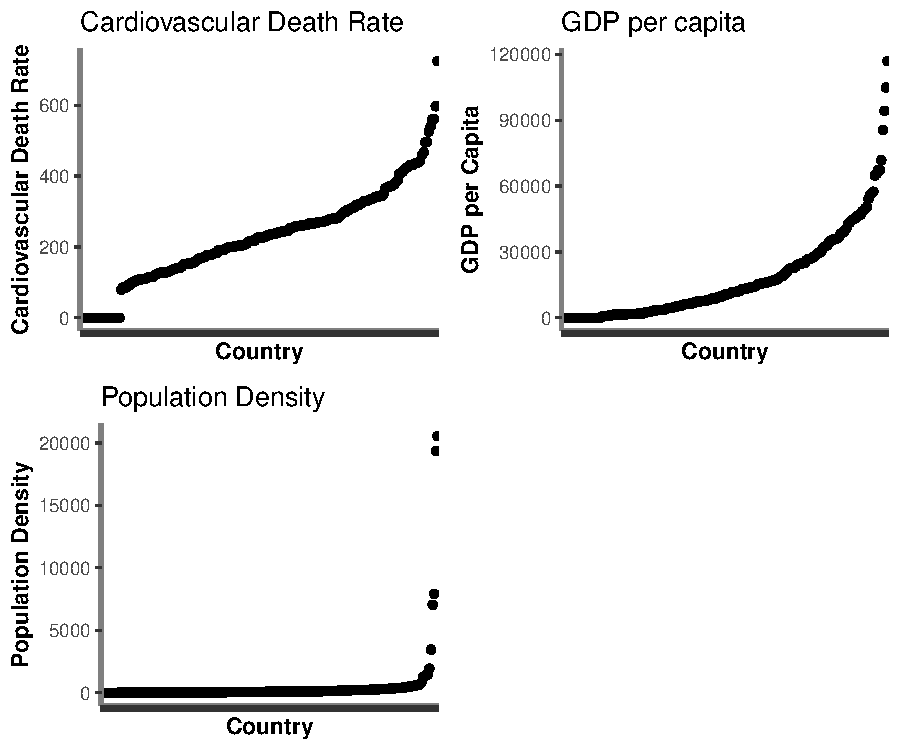
\includegraphics{Cross_Section_Assignment_files/figure-latex/cons_plot-1.pdf}

\begin{Shaded}
\begin{Highlighting}[]
\NormalTok{world\_df }\OtherTok{\textless{}{-}}\NormalTok{ world\_df }\SpecialCharTok{\%\textgreater{}\%} \FunctionTok{scale\_bigs\_constant}\NormalTok{(.)}
\end{Highlighting}
\end{Shaded}

Now we can check all the descriptive stats for all the columns

\begin{verbatim}
##                                    mean         sd   min         max
## new_cases                     261519.32 1220518.92  0.00 25275423.00
## afflicted_rate                    26.00      85.81  0.00      931.54
## reproduction_rate                  0.77       0.44 -0.01        2.06
## stringency_index                  44.81      25.15  0.00       99.06
## median_age                        27.58      12.79  0.00       48.20
## aged_65_older                      7.90       6.48  0.00       27.05
## extreme_poverty                    7.83      16.76  0.00       77.60
## diabetes_prevalence                7.52       4.59  0.00       23.36
## handwashing_facilities            21.89      32.72  0.00       99.00
## hosp_beds_1k                       2.38       2.51  0.00       13.80
## life_expectancy                   73.36       9.08  0.00       86.75
## human_development_index           62.94      28.48  0.00       95.70
## smokers                           14.38      12.75  0.00       45.95
## new_vaccinations_cum_per_1000      0.00       1.00 -0.49        4.95
## new_tests_cum_per_1000             0.00       1.00 -0.27       18.13
## population_density_norm            0.00       1.00 -0.21        9.60
## cardiovasc_death_rate_norm         0.00       1.00 -1.67        3.69
## gdp_per_capita_log                 8.21       3.22  0.00       11.67
##                                     range
## new_cases                     25275423.00
## afflicted_rate                     931.54
## reproduction_rate                    2.08
## stringency_index                    99.06
## median_age                          48.20
## aged_65_older                       27.05
## extreme_poverty                     77.60
## diabetes_prevalence                 23.36
## handwashing_facilities              99.00
## hosp_beds_1k                        13.80
## life_expectancy                     86.75
## human_development_index             95.70
## smokers                             45.95
## new_vaccinations_cum_per_1000        5.45
## new_tests_cum_per_1000              18.40
## population_density_norm              9.81
## cardiovasc_death_rate_norm           5.36
## gdp_per_capita_log                  11.67
\end{verbatim}

The value of the stringency index is assumed to have a delayed effect on
the coronavirus, therefore, to account for this, one quarter lagged
average stringency index value is associated the current with each
current period.

\begin{Shaded}
\begin{Highlighting}[]
\NormalTok{world\_df }\OtherTok{\textless{}{-}}\NormalTok{ world\_df }\SpecialCharTok{\%\textgreater{}\%}
    \FunctionTok{group\_by}\NormalTok{(location) }\SpecialCharTok{\%\textgreater{}\%}
    \FunctionTok{mutate}\NormalTok{(}\FunctionTok{across}\NormalTok{(date, }\ControlFlowTok{function}\NormalTok{(x) }\FunctionTok{floor\_date}\NormalTok{(x, }\AttributeTok{unit =} \StringTok{"quarters"}\NormalTok{))) }\SpecialCharTok{\%\textgreater{}\%} 
    \FunctionTok{ungroup}\NormalTok{()}
    
\NormalTok{quick\_df }\OtherTok{\textless{}{-}}\NormalTok{ world\_df }\SpecialCharTok{\%\textgreater{}\%}
    \FunctionTok{select}\NormalTok{(location, date, stringency\_index) }\SpecialCharTok{\%\textgreater{}\%} 
    \FunctionTok{group\_by}\NormalTok{(location) }\SpecialCharTok{\%\textgreater{}\%} 
    \FunctionTok{mutate}\NormalTok{(}\FunctionTok{across}\NormalTok{(date, }\ControlFlowTok{function}\NormalTok{(x) x }\SpecialCharTok{\%m+\%} \FunctionTok{months}\NormalTok{(}\DecValTok{3}\NormalTok{))) }\SpecialCharTok{\%\textgreater{}\%} 
    \FunctionTok{filter}\NormalTok{(date }\SpecialCharTok{!=} \FunctionTok{last}\NormalTok{(date))}

\NormalTok{world\_df }\OtherTok{\textless{}{-}}\NormalTok{ quick\_df }\SpecialCharTok{\%\textgreater{}\%} \FunctionTok{left\_join}\NormalTok{(world\_df, }\AttributeTok{by =} \FunctionTok{c}\NormalTok{(}\StringTok{"location"}\NormalTok{, }\StringTok{"date"}\NormalTok{)) }\SpecialCharTok{\%\textgreater{}\%} 
    \FunctionTok{select}\NormalTok{(}\SpecialCharTok{{-}}\NormalTok{stringency\_index.y)}
\end{Highlighting}
\end{Shaded}

\hypertarget{correlation-analysis}{%
\section{Correlation Analysis}\label{correlation-analysis}}

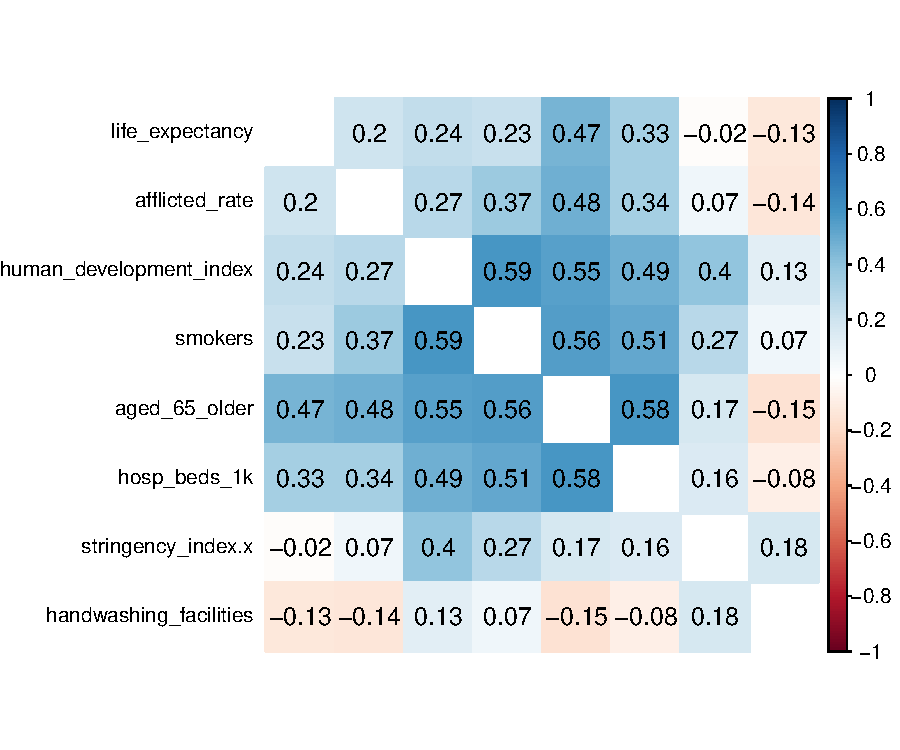
\includegraphics{Cross_Section_Assignment_files/figure-latex/cor_plot-1.pdf}

\begin{verbatim}
## [1] "full"
\end{verbatim}

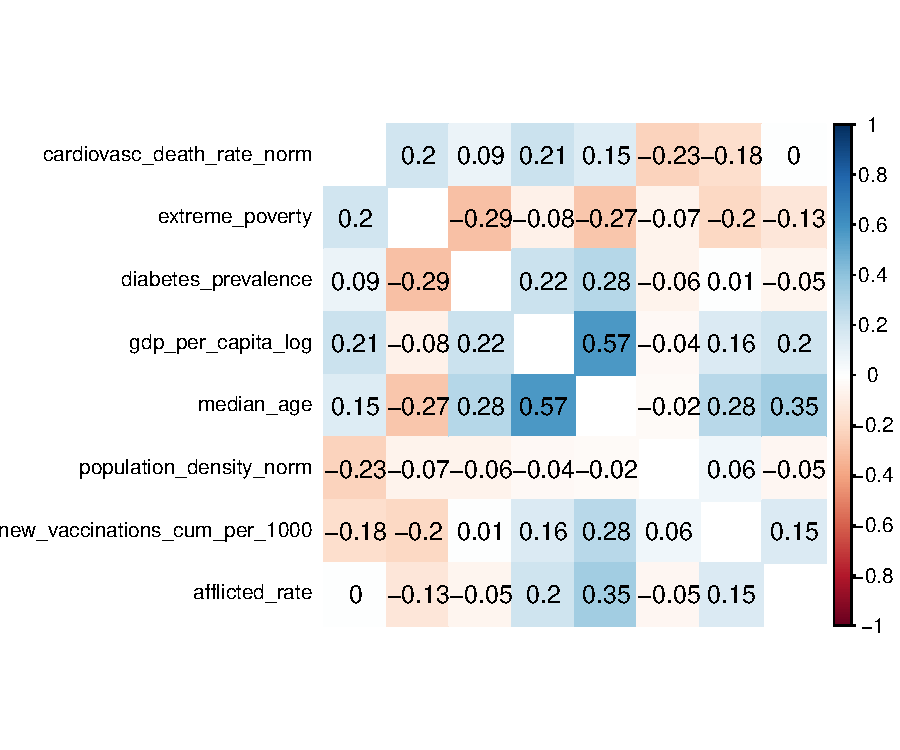
\includegraphics{Cross_Section_Assignment_files/figure-latex/core_plot2-1.pdf}

\begin{verbatim}
## [1] "full"
\end{verbatim}

The components that will form a part of the larger OLS regression is
therefore the:

\begin{itemize}
\tightlist
\item
  stringency index \texttt{stringency\_index.x}
\end{itemize}

\begin{itemize}
\item
  development index \texttt{human\_development\_index}
\item
  proportion of smokers \texttt{smokers}
\item
  population over the age of 65 \texttt{aged\_65\_older}
\item
  and hospital beds per 1000 \texttt{hosp\_beds\_1k}
\item
  Availability of hand washing facilities
  \texttt{handwashing\_facilities}
\end{itemize}

Hand washing facilities is added based on intuitive interpretation

\hypertarget{regressions}{%
\section{Regressions}\label{regressions}}

\hypertarget{ols-regression}{%
\subsection{OLS Regression}\label{ols-regression}}

\begin{Shaded}
\begin{Highlighting}[]
\NormalTok{mod\_ols\_1 }\OtherTok{\textless{}{-}} \FunctionTok{plm}\NormalTok{(afflicted\_rate }\SpecialCharTok{\textasciitilde{}}\NormalTok{ stringency\_index.x }\SpecialCharTok{+}
\NormalTok{   handwashing\_facilities }\SpecialCharTok{+}\NormalTok{ reproduction\_rate,}
    \AttributeTok{index =} \FunctionTok{c}\NormalTok{(}\StringTok{"location"}\NormalTok{, }\StringTok{"date"}\NormalTok{), }\AttributeTok{data =}\NormalTok{ world\_df, }
   \AttributeTok{model =} \StringTok{"pooling"}\NormalTok{)}

\NormalTok{mod\_ols\_2 }\OtherTok{\textless{}{-}} \FunctionTok{plm}\NormalTok{(afflicted\_rate }\SpecialCharTok{\textasciitilde{}}\NormalTok{ stringency\_index.x }\SpecialCharTok{+}\NormalTok{ smokers}
   \SpecialCharTok{+}\NormalTok{ handwashing\_facilities }\SpecialCharTok{+}\NormalTok{ aged\_65\_older }\SpecialCharTok{+}\NormalTok{ hosp\_beds\_1k}
   \SpecialCharTok{+}\NormalTok{ human\_development\_index }\SpecialCharTok{+}\NormalTok{ reproduction\_rate, }
   \AttributeTok{data =}\NormalTok{ world\_df, }
   \AttributeTok{index =} \FunctionTok{c}\NormalTok{(}\StringTok{"location"}\NormalTok{, }\StringTok{"date"}\NormalTok{), }\AttributeTok{model =} \StringTok{"pooling"}\NormalTok{)}

\NormalTok{mod\_1sls }\OtherTok{\textless{}{-}} \FunctionTok{plm}\NormalTok{(stringency\_index.x }\SpecialCharTok{\textasciitilde{}}\NormalTok{ gdp\_per\_capita\_log,}
                \AttributeTok{data =}\NormalTok{ world\_df, }
                \AttributeTok{index =} \FunctionTok{c}\NormalTok{(}\StringTok{"location"}\NormalTok{, }\StringTok{"date"}\NormalTok{), }\AttributeTok{model =} \StringTok{"pooling"}\NormalTok{)}

\NormalTok{stringency\_hat }\OtherTok{\textless{}{-}} \FunctionTok{fitted.values}\NormalTok{(mod\_1sls)}

\NormalTok{mod\_2sls }\OtherTok{\textless{}{-}} \FunctionTok{plm}\NormalTok{(afflicted\_rate }\SpecialCharTok{\textasciitilde{}}\NormalTok{ stringency\_hat }\SpecialCharTok{+}\NormalTok{ smokers}
   \SpecialCharTok{+}\NormalTok{ handwashing\_facilities }\SpecialCharTok{+}\NormalTok{ aged\_65\_older }\SpecialCharTok{+}\NormalTok{ hosp\_beds\_1k}
   \SpecialCharTok{+}\NormalTok{ human\_development\_index, }
   \AttributeTok{data =}\NormalTok{ world\_df, }
   \AttributeTok{index =} \FunctionTok{c}\NormalTok{(}\StringTok{"location"}\NormalTok{, }\StringTok{"date"}\NormalTok{), }\AttributeTok{model =} \StringTok{"pooling"}\NormalTok{)}

\CommentTok{\# To get robust standard errors}
\NormalTok{robustse\_ols1 }\OtherTok{\textless{}{-}} \FunctionTok{sqrt}\NormalTok{(}\FunctionTok{diag}\NormalTok{(}\FunctionTok{vcovHC}\NormalTok{(mod\_ols\_1, }\AttributeTok{type =} \StringTok{"HC1"}\NormalTok{)))}
\NormalTok{robustse\_ols2 }\OtherTok{\textless{}{-}} \FunctionTok{sqrt}\NormalTok{(}\FunctionTok{diag}\NormalTok{(}\FunctionTok{vcovHC}\NormalTok{(mod\_ols\_2, }\AttributeTok{type =} \StringTok{"HC1"}\NormalTok{)))}
\NormalTok{robustse\_2sls }\OtherTok{\textless{}{-}} \FunctionTok{sqrt}\NormalTok{(}\FunctionTok{diag}\NormalTok{(}\FunctionTok{vcovHC}\NormalTok{(mod\_2sls, }\AttributeTok{type =} \StringTok{"HC1"}\NormalTok{)))}
\end{Highlighting}
\end{Shaded}

\begin{Shaded}
\begin{Highlighting}[]
\FunctionTok{stargazer}\NormalTok{(mod\_ols\_1, mod\_ols\_2, mod\_2sls, }\AttributeTok{header =}\NormalTok{ F, }\AttributeTok{font.size =} \StringTok{"footnotesize"}\NormalTok{,}
    \AttributeTok{se =} \FunctionTok{list}\NormalTok{(robustse\_ols1, robustse\_ols2, robustse\_2sls), }\AttributeTok{column.labels =} \FunctionTok{c}\NormalTok{(}\StringTok{"OLS"}\NormalTok{,}
        \StringTok{"OLS"}\NormalTok{, }\StringTok{"2SLS"}\NormalTok{))}
\end{Highlighting}
\end{Shaded}

\begin{table}[!htbp] \centering 
  \caption{} 
  \label{} 
\footnotesize 
\begin{tabular}{@{\extracolsep{5pt}}lccc} 
\\[-1.8ex]\hline 
\hline \\[-1.8ex] 
 & \multicolumn{3}{c}{\textit{Dependent variable:}} \\ 
\cline{2-4} 
\\[-1.8ex] & \multicolumn{3}{c}{afflicted\_rate} \\ 
 & OLS & OLS & 2SLS \\ 
\\[-1.8ex] & (1) & (2) & (3)\\ 
\hline \\[-1.8ex] 
 stringency\_index.x & 0.072 & $-$0.108 &  \\ 
  & (0.096) & (0.112) &  \\ 
  & & & \\ 
 stringency\_hat &  &  & $-$0.101 \\ 
  &  &  & (0.395) \\ 
  & & & \\ 
 smokers &  & 1.139$^{***}$ & 1.136$^{***}$ \\ 
  &  & (0.431) & (0.426) \\ 
  & & & \\ 
 handwashing\_facilities & $-$0.474$^{***}$ & $-$0.226 & $-$0.226 \\ 
  & (0.172) & (0.152) & (0.150) \\ 
  & & & \\ 
 aged\_65\_older &  & 5.211$^{***}$ & 5.155$^{***}$ \\ 
  &  & (0.914) & (0.931) \\ 
  & & & \\ 
 hosp\_beds\_1k &  & 1.727 & 1.841 \\ 
  &  & (2.473) & (2.496) \\ 
  & & & \\ 
 human\_development\_index &  & $-$0.187 & $-$0.105 \\ 
  &  & (0.177) & (0.198) \\ 
  & & & \\ 
 reproduction\_rate & 39.621$^{***}$ & 10.297$^{**}$ &  \\ 
  & (7.000) & (4.454) &  \\ 
  & & & \\ 
 Constant & 3.190 & $-$19.596$^{***}$ & $-$16.447 \\ 
  & (2.717) & (5.501) & (13.190) \\ 
  & & & \\ 
\hline \\[-1.8ex] 
Observations & 1,844 & 1,844 & 1,844 \\ 
R$^{2}$ & 0.054 & 0.256 & 0.255 \\ 
Adjusted R$^{2}$ & 0.052 & 0.253 & 0.252 \\ 
F Statistic & 34.712$^{***}$ (df = 3; 1840) & 90.259$^{***}$ (df = 7; 1836) & 104.560$^{***}$ (df = 6; 1837) \\ 
\hline 
\hline \\[-1.8ex] 
\textit{Note:}  & \multicolumn{3}{r}{$^{*}$p$<$0.1; $^{**}$p$<$0.05; $^{***}$p$<$0.01} \\ 
\end{tabular} 
\end{table}

\hypertarget{fixed--and-random-effects-regression}{%
\subsection{Fixed- and Random Effects
Regression}\label{fixed--and-random-effects-regression}}

\begin{Shaded}
\begin{Highlighting}[]
\NormalTok{mod\_fe\_1 }\OtherTok{\textless{}{-}} \FunctionTok{plm}\NormalTok{(afflicted\_rate }\SpecialCharTok{\textasciitilde{}}\NormalTok{ stringency\_index.x }\SpecialCharTok{+}\NormalTok{ smokers}
   \SpecialCharTok{+}\NormalTok{ handwashing\_facilities }\SpecialCharTok{+}\NormalTok{ aged\_65\_older }\SpecialCharTok{+}\NormalTok{ hosp\_beds\_1k}
   \SpecialCharTok{+}\NormalTok{ human\_development\_index, }
   \AttributeTok{data =}\NormalTok{ world\_df, }
   \AttributeTok{index =} \FunctionTok{c}\NormalTok{(}\StringTok{"location"}\NormalTok{), }
  \AttributeTok{model =} \StringTok{"within"}\NormalTok{, }\AttributeTok{effect =} \StringTok{"individual"}\NormalTok{)}


\NormalTok{robustse\_fe1 }\OtherTok{\textless{}{-}} \FunctionTok{sqrt}\NormalTok{(}\FunctionTok{diag}\NormalTok{(}\FunctionTok{vcovHC}\NormalTok{(mod\_fe\_1, }\AttributeTok{type =} \StringTok{"HC1"}\NormalTok{)))}
\end{Highlighting}
\end{Shaded}

\begin{Shaded}
\begin{Highlighting}[]
\NormalTok{mod\_re\_1 }\OtherTok{\textless{}{-}} \FunctionTok{plm}\NormalTok{(afflicted\_rate }\SpecialCharTok{\textasciitilde{}}\NormalTok{ stringency\_index.x }\SpecialCharTok{+}\NormalTok{ smokers}
   \SpecialCharTok{+}\NormalTok{ handwashing\_facilities }\SpecialCharTok{+}\NormalTok{ aged\_65\_older }\SpecialCharTok{+}\NormalTok{ hosp\_beds\_1k}
   \SpecialCharTok{+}\NormalTok{ human\_development\_index,}
                   \AttributeTok{data =}\NormalTok{ world\_df,}
                   \AttributeTok{index =} \FunctionTok{c}\NormalTok{(}\StringTok{"location"}\NormalTok{),}
                  \AttributeTok{model =} \StringTok{"random"}\NormalTok{)}

\NormalTok{robustse\_re1 }\OtherTok{\textless{}{-}} \FunctionTok{sqrt}\NormalTok{(}\FunctionTok{diag}\NormalTok{(}\FunctionTok{vcovHC}\NormalTok{(mod\_re\_1, }\AttributeTok{type =} \StringTok{"HC1"}\NormalTok{)))}
\end{Highlighting}
\end{Shaded}

\begin{Shaded}
\begin{Highlighting}[]
\FunctionTok{stargazer}\NormalTok{(mod\_fe\_1, mod\_re\_1, }\AttributeTok{header =}\NormalTok{ F, }\AttributeTok{font.size =} \StringTok{"small"}\NormalTok{, }\AttributeTok{se =} \FunctionTok{list}\NormalTok{(robustse\_re1),}
    \AttributeTok{column.labels =} \FunctionTok{c}\NormalTok{(}\StringTok{"FE"}\NormalTok{, }\StringTok{"RE"}\NormalTok{))}
\end{Highlighting}
\end{Shaded}

\begin{table}[!htbp] \centering 
  \caption{} 
  \label{} 
\small 
\begin{tabular}{@{\extracolsep{5pt}}lcc} 
\\[-1.8ex]\hline 
\hline \\[-1.8ex] 
 & \multicolumn{2}{c}{\textit{Dependent variable:}} \\ 
\cline{2-3} 
\\[-1.8ex] & \multicolumn{2}{c}{afflicted\_rate} \\ 
 & FE & RE \\ 
\\[-1.8ex] & (1) & (2)\\ 
\hline \\[-1.8ex] 
 stringency\_index.x & $-$0.095 & $-$0.088 \\ 
  & (0.072) & (0.094) \\ 
  & & \\ 
 smokers &  & 1.155$^{***}$ \\ 
  &  & (0.413) \\ 
  & & \\ 
 handwashing\_facilities &  & $-$0.219$^{*}$ \\ 
  &  & (0.126) \\ 
  & & \\ 
 aged\_65\_older &  & 5.125$^{***}$ \\ 
  &  & (0.846) \\ 
  & & \\ 
 hosp\_beds\_1k &  & 1.830 \\ 
  &  & (2.013) \\ 
  & & \\ 
 human\_development\_index &  & $-$0.105 \\ 
  &  & (0.187) \\ 
  & & \\ 
 Constant &  & $-$17.164$^{*}$ \\ 
  &  & (9.821) \\ 
  & & \\ 
\hline \\[-1.8ex] 
Observations & 1,844 & 1,844 \\ 
R$^{2}$ & 0.0005 & 0.069 \\ 
Adjusted R$^{2}$ & $-$0.125 & 0.066 \\ 
F Statistic & 0.819 (df = 1; 1637) & 137.243$^{***}$ \\ 
\hline 
\hline \\[-1.8ex] 
\textit{Note:}  & \multicolumn{2}{r}{$^{*}$p$<$0.1; $^{**}$p$<$0.05; $^{***}$p$<$0.01} \\ 
\end{tabular} 
\end{table}

\hypertarget{interpretations}{%
\subsection{Interpretations}\label{interpretations}}

\hypertarget{measurement-error-bias}{%
\subsubsection{Measurement Error \& Bias}\label{measurement-error-bias}}

It is important to note that the unexpected nature of Covid-19 resulted
in a lot of ``on the fly'' data collection which can lead to larger
measurement errors. The reliability of measurement error and false
estimates in this case is questionable. Furthermore, the fixed- and
random effects regressions can exacerbate this problem. In that case, it
would suggest that a pooled OLS regression offer some particular
benefits.

\hypertarget{assumptions-of-ols}{%
\subsubsection{Assumptions of OLS:}\label{assumptions-of-ols}}

There exists an inherent endogeneity in this dataset, since there exists
some country specific factors that might have led to lockdowns being
more effective or having more resources to withstand the aderse effects
of lockowns. For this reason, the last OLS model includes a two stage
least squares regression model to mitigate this issue. Additionally, the
Random- and Fixed effects models are also fitted. These can more
precisely account for country specific factors playing a role.

The Instrumental Variable regression, by method of two stage least
squares, requires the following assumptions to hold for an unbiased
estimate:

Instrument Variable: reproduction rate, such that it affects the
afflicted rate stringency through the stringency index

\begin{enumerate}
\def\labelenumi{\arabic{enumi}.}
\tightlist
\item
  Exclusion Restriction
\end{enumerate}

This requires that the reproduction rate only affects the afflicted rate
through the stringency index.

This assumption is less likely to hold. however, since the assumption is
that the degree of harm that the virus inflicts should reduce even if
the infectiousness rises due to vaccinations etc. There is still a
possibility that this might hold. Also, the expection is that if
lockdowns are reasonably effective, that the contagiousness of the virus
should not affect the afflicted rate per ten thousand individuals in the
population.

\begin{enumerate}
\def\labelenumi{\arabic{enumi}.}
\setcounter{enumi}{1}
\tightlist
\item
  Random Assignment
\end{enumerate}

This requires that there be no difference between the potential outcomes

\hypertarget{assumptions-of-fixed--and-random-effects}{%
\subsubsection{Assumptions of Fixed- and Random
Effects}\label{assumptions-of-fixed--and-random-effects}}

\hypertarget{references}{%
\section{References}\label{references}}

\hypertarget{refs}{}
\begin{CSLReferences}{1}{0}
\leavevmode\vadjust pre{\hypertarget{ref-dataset}{}}%
H. Ritchie, L.R.-G., E. Mathieu. 2020. Coronavirus pandemic (COVID-19).
\emph{Our World in Data}.

\end{CSLReferences}

\hypertarget{appendix}{%
\section{Appendix}\label{appendix}}

\begin{Shaded}
\begin{Highlighting}[]
\CommentTok{\# Checking the date of first observations}
\FunctionTok{start\_date}\NormalTok{()}


\CommentTok{\# fetching and cleaning the dataset}
\NormalTok{world\_df }\OtherTok{\textless{}{-}} \FunctionTok{extract\_all}\NormalTok{() }\SpecialCharTok{\%\textgreater{}\%} 
    \FunctionTok{feature\_adj\_all}\NormalTok{() }\SpecialCharTok{\%\textgreater{}\%} 
    \FunctionTok{experiment\_aggregate\_week}\NormalTok{() }\SpecialCharTok{\%\textgreater{}\%} 
    \FunctionTok{experiment\_trim}\NormalTok{() }\SpecialCharTok{\%\textgreater{}\%} 
    \FunctionTok{relocate}\NormalTok{(afflicted\_rate, }\AttributeTok{.before =}\NormalTok{ reproduction\_rate)}

\NormalTok{world\_df}
\CommentTok{\# See appendix}
\NormalTok{world\_df }\OtherTok{\textless{}{-}}\NormalTok{ world\_df }\SpecialCharTok{\%\textgreater{}\%} \FunctionTok{scale\_bigs\_cumsum}\NormalTok{(.)}
\NormalTok{world\_df }\OtherTok{\textless{}{-}}\NormalTok{ world\_df }\SpecialCharTok{\%\textgreater{}\%}
    \FunctionTok{group\_by}\NormalTok{(location) }\SpecialCharTok{\%\textgreater{}\%}
    \FunctionTok{mutate}\NormalTok{(}\FunctionTok{across}\NormalTok{(date, }\ControlFlowTok{function}\NormalTok{(x) }\FunctionTok{floor\_date}\NormalTok{(x, }\AttributeTok{unit =} \StringTok{"quarters"}\NormalTok{))) }\SpecialCharTok{\%\textgreater{}\%} 
    \FunctionTok{ungroup}\NormalTok{()}
    
\NormalTok{quick\_df }\OtherTok{\textless{}{-}}\NormalTok{ world\_df }\SpecialCharTok{\%\textgreater{}\%}
    \FunctionTok{select}\NormalTok{(location, date, stringency\_index) }\SpecialCharTok{\%\textgreater{}\%} 
    \FunctionTok{group\_by}\NormalTok{(location) }\SpecialCharTok{\%\textgreater{}\%} 
    \FunctionTok{mutate}\NormalTok{(}\FunctionTok{across}\NormalTok{(date, }\ControlFlowTok{function}\NormalTok{(x) x }\SpecialCharTok{\%m+\%} \FunctionTok{months}\NormalTok{(}\DecValTok{3}\NormalTok{))) }\SpecialCharTok{\%\textgreater{}\%} 
    \FunctionTok{filter}\NormalTok{(date }\SpecialCharTok{!=} \FunctionTok{last}\NormalTok{(date))}

\NormalTok{world\_df }\OtherTok{\textless{}{-}}\NormalTok{ quick\_df }\SpecialCharTok{\%\textgreater{}\%} \FunctionTok{left\_join}\NormalTok{(world\_df, }\AttributeTok{by =} \FunctionTok{c}\NormalTok{(}\StringTok{"location"}\NormalTok{, }\StringTok{"date"}\NormalTok{)) }\SpecialCharTok{\%\textgreater{}\%} 
    \FunctionTok{select}\NormalTok{(}\SpecialCharTok{{-}}\NormalTok{stringency\_index.y)}
\FunctionTok{cor\_plot2}\NormalTok{(world\_df)}\SpecialCharTok{$}\NormalTok{arg}\SpecialCharTok{$}\NormalTok{type}
\FunctionTok{names}\NormalTok{(world\_df)}
\end{Highlighting}
\end{Shaded}

\hypertarget{functional-code}{%
\subsection{Functional Code}\label{functional-code}}

\begin{verbatim}
## function (df) 
## {
##     plot <- df %>% ggplot(aes(fill = location, y = afflicted_rate/206, 
##         x = date)) + geom_area(position = "stack", stat = "identity", 
##         alpha = 0.5) + theme(legend.position = "none") + theme(axis.text.x = element_text(size = 10), 
##         axis.title = element_text(face = "bold"), axis.line = element_line(colour = "grey50", 
##             size = 1)) + scale_y_continuous("Afflicated Rate")
##     return(plot)
## }
\end{verbatim}

\begin{verbatim}
## function (df) 
## {
##     plot <- df %>% ungroup() %>% group_by(location) %>% filter(date == 
##         last(date)) %>% ggplot() + geom_point(aes(x = reorder(location, 
##         cardiovasc_death_rate, mean), y = cardiovasc_death_rate)) + 
##         theme(axis.text.x = element_blank(), axis.title = element_text(face = "bold"), 
##             axis.line = element_line(colour = "grey50", size = 1)) + 
##         scale_y_continuous("Cardiovascular Death Rate") + scale_x_discrete("Country") + 
##         labs(title = "Cardiovascular Death Rate")
##     return(plot)
## }
\end{verbatim}

\begin{verbatim}
## function (df, constant_features = c("gdp_per_capita", "population_density", 
##     "median_age", "aged_65_older", "extreme_poverty", "cardiovasc_death_rate", 
##     "diabetes_prevalence", "handwashing_facilities", "hosp_beds_1k", 
##     "life_expectancy", "human_development_index", "smokers")) 
## {
##     descriptive_stats <- df %>% ungroup() %>% select(-c(constant_features, 
##         date, location)) %>% describe() %>% select(-c(median, 
##         mad, se, vars, n, skew, kurtosis, trimmed))
##     return(descriptive_stats)
## }
## <bytecode: 0x000001d6de8c0650>
\end{verbatim}

\begin{verbatim}
## function (df, constant_features = c("gdp_per_capita", "population_density", 
##     "median_age", "aged_65_older", "extreme_poverty", "cardiovasc_death_rate", 
##     "diabetes_prevalence", "handwashing_facilities", "hosp_beds_1k", 
##     "life_expectancy", "human_development_index", "smokers")) 
## {
##     descriptive_stats <- df %>% ungroup() %>% select(constant_features) %>% 
##         describe() %>% select(-c(median, mad, se, vars, n, skew, 
##         kurtosis, trimmed))
##     return(descriptive_stats)
## }
\end{verbatim}

\begin{verbatim}
## function (df) 
## {
##     plot1 <- df %>% ungroup() %>% select(-c(location, date, gdp_per_capita_log, 
##         population_density_norm, cardiovasc_death_rate_norm, 
##         reproduction_rate, new_tests_cum_per_1000, new_vaccinations_cum_per_1000, 
##         median_age, extreme_poverty, diabetes_prevalence, new_cases, 
##         reproduction_rate, new_cases)) %>% cor(.)
##     plot2 <- plot1 %>% corrplot(., method = "color", order = "hclust", 
##         tl.srt = 0, diag = F, tl.col = "black", addCoef.col = "black", 
##         tl.pos = "l", tl.cex = 0.8, number.font = 8)
##     return(plot2)
## }
\end{verbatim}

\begin{verbatim}
## function (df) 
## {
##     plot1 <- df %>% ungroup() %>% select(c(gdp_per_capita_log, 
##         population_density_norm, cardiovasc_death_rate_norm, 
##         new_vaccinations_cum_per_1000, median_age, extreme_poverty, 
##         diabetes_prevalence, afflicted_rate)) %>% cor(.)
##     plot2 <- plot1 %>% corrplot(., method = "color", order = "hclust", 
##         tl.srt = 0, diag = F, tl.col = "black", addCoef.col = "black", 
##         tl.pos = "l", tl.cex = 0.8, number.font = 8)
##     return(plot2)
## }
\end{verbatim}

\begin{verbatim}
## function (df) 
## {
##     plot <- world_df %>% ungroup() %>% group_by(location) %>% 
##         mutate(label = if_else(date == last(date), as.character(location), 
##             NA_character_)) %>% ggplot(aes(x = date, y = new_tests, 
##         group = location, col = location)) + geom_line() + theme(axis.text.x = element_blank(), 
##         axis.title = element_text(face = "bold"), axis.line = element_line(colour = "grey50", 
##             size = 1)) + scale_y_continuous("cumulative Vaccines per Thousand") + 
##         geom_label_repel(aes(label = label), nudge_x = 1, na.rm = TRUE) + 
##         theme(legend.position = "none")
##     return(plot)
## }
## <bytecode: 0x000001d6dd1fe618>
\end{verbatim}

\begin{verbatim}
## function (df) 
## {
##     plot <- df %>% ungroup() %>% group_by(location) %>% mutate(label = if_else(date == 
##         last(date), as.character(location), NA_character_)) %>% 
##         ggplot(aes(x = date, y = new_tests, group = location, 
##             col = location)) + geom_line() + theme(axis.text.x = element_blank(), 
##         axis.title = element_text(face = "bold"), axis.line = element_line(colour = "grey50", 
##             size = 1)) + scale_y_continuous("cumulative Tests per Thousand") + 
##         geom_label_repel(aes(label = label), nudge_x = 1, na.rm = TRUE) + 
##         theme(legend.position = "none")
##     return(plot)
## }
## <bytecode: 0x000001d6f4e92e20>
\end{verbatim}

\begin{verbatim}
## function (df) 
## {
##     constant_features <- c("gdp_per_capita", "population_density", 
##         "median_age", "aged_65_older", "extreme_poverty", "cardiovasc_death_rate", 
##         "diabetes_prevalence", "handwashing_facilities", "hosp_beds_1k", 
##         "life_expectancy", "human_development_index", "smokers", 
##         "population")
##     mean_cols = c("reproduction_rate", "stringency_index")
##     df <- df %>% replace(is.na(.), 0) %>% select(-excess_mortality) %>% 
##         mutate(year_quarter = paste(year(date), quarter(date), 
##             sep = "-")) %>% relocate(year_quarter, .before = date) %>% 
##         group_by(location, year_quarter) %>% mutate(across(-c(constant_features, 
##         mean_cols, date), sum), across(c(mean_cols), function(x) mean(x))) %>% 
##         ungroup()
##     return(df)
## }
## <bytecode: 0x000001d6df16a5b8>
\end{verbatim}

\begin{verbatim}
## function (df) 
## {
##     df <- df %>% group_by(location, year_quarter) %>% filter(row_number() == 
##         n()) %>% ungroup() %>% select(-c(year_quarter)) %>% group_by(location, 
##         date) %>% mutate(afflicted_rate = ((new_deaths + icu_patients + 
##         hosp_patients)/population * 10000), .keep = "unused") %>% 
##         replace(is.na(.), 0)
##     return(df)
## }
\end{verbatim}

\begin{verbatim}
## function (path = "./data/owid-covid-data.csv") 
## {
##     names1 <- c(".+smoothed.*", ".+per_million", ".+per_thousand", 
##         ".+per_hundred", ".*cumulative.*", ".*weekly.*", "total.+")
##     continents <- extract_continents()$continent
##     df <- read_csv(file = path, show_col_types = F) %>% filter(!location %in% 
##         c(continents)) %>% filter(!is.na(continent)) %>% group_by(location) %>% 
##         filter(first(date) <= lubridate::ymd(20200430)) %>% ungroup() %>% 
##         select(-c(iso_code, continent, tests_units)) %>% rename(hosp_beds_1k = hospital_beds_per_thousand) %>% 
##         .[, !grepl(names(.), pattern = paste(names1, collapse = "|"))]
##     return(df)
## }
## <bytecode: 0x000001d6ddb77ae0>
\end{verbatim}

\begin{verbatim}
## function (path = "./data/owid-covid-data.csv") 
## {
##     continents <- read_csv(file = path, show_col_types = F) %>% 
##         select(continent) %>% unique()
##     return(continents)
## }
\end{verbatim}

\begin{verbatim}
## function (df) 
## {
##     df %<>% mutate(new_vaccinations = (new_vaccinations/population) * 
##         1000) %>% mutate(new_tests = (new_tests/population) * 
##         1000) %>% select(-c(aged_70_older, people_fully_vaccinated, 
##         people_vaccinated, tests_per_case, positive_rate)) %>% 
##         group_by(location) %>% mutate(smokers = mean(c(female_smokers, 
##         male_smokers)), .keep = "unused")
##     return(df)
## }
\end{verbatim}

\begin{verbatim}
## function (df) 
## {
##     plot <- df %>% ungroup() %>% group_by(location) %>% filter(date == 
##         last(date)) %>% ggplot() + geom_point(aes(x = reorder(location, 
##         gdp_per_capita, mean), y = gdp_per_capita)) + theme(axis.text.x = element_blank(), 
##         axis.title = element_text(face = "bold"), axis.line = element_line(colour = "grey50", 
##             size = 1)) + scale_y_continuous("GDP per Capita") + 
##         scale_x_discrete("Country") + labs(title = "GDP per capita")
##     return(plot)
## }
\end{verbatim}

\begin{verbatim}
## function (df) 
## {
##     plot <- df %>% ungroup() %>% group_by(location) %>% filter(date == 
##         last(date)) %>% ggplot() + geom_point(aes(x = reorder(location, 
##         population_density, mean), y = population_density)) + 
##         theme(axis.text.x = element_blank(), axis.title = element_text(face = "bold"), 
##             axis.line = element_line(colour = "grey50", size = 1)) + 
##         scale_y_continuous("Population Density") + scale_x_discrete("Country") + 
##         labs(title = "Population Density")
##     return(plot)
## }
\end{verbatim}

\begin{verbatim}
## function (df) 
## {
##     df <- df %>% ungroup() %>% mutate(across(c("population_density", 
##         "cardiovasc_death_rate"), function(x) scale(x, center = T), 
##         .names = "{.col}_norm"), across(c("gdp_per_capita"), 
##         function(x) if_else(x == 0, 0, log(x)), .names = "{.col}_log"), 
##         across(c("human_development_index"), function(x) x * 
##             100, .names = "{.col}"), .keep = "unused")
##     return(df)
## }
\end{verbatim}

\begin{verbatim}
## function (df, big_cols = c("new_tests", "new_vaccinations")) 
## {
##     df <- df %>% ungroup() %>% group_by(location) %>% mutate(across(big_cols, 
##         function(x) cumsum(x), .names = "{.col}"), .keep = "unused") %>% 
##         return(df)
## }
\end{verbatim}

\begin{verbatim}
## function (df, big_cols = c("new_vaccinations", "new_tests")) 
## {
##     df <- df %>% ungroup() %>% mutate(across(big_cols, function(x) scale(x), 
##         .names = "{.col}_cum_per_1000"), .keep = "unused")
##     return(df)
## }
\end{verbatim}

\begin{verbatim}
## function () 
## {
##     plot <- read_csv(file = "./data/owid-covid-data.csv", show_col_types = F) %>% 
##         group_by(location) %>% filter(date == first(date)) %>% 
##         ggplot() + geom_point(aes(x = location, y = date)) + 
##         geom_hline(yintercept = lubridate::ymd(20200430), color = "red") + 
##         theme(axis.text.x = element_blank(), axis.title = element_text(face = "bold"), 
##             axis.line = element_line(colour = "grey50", size = 1)) + 
##         scale_y_date("First Date Observation")
##     return(plot)
## }
\end{verbatim}

\bibliography{Tex/ref}





\end{document}
